\newpage % Rozdziały zaczynamy od nowej strony.
 

\section{Implementacja wtyczki}
\begin{description}
\item[Zintegrowane środowisko programistyczne Sublime Text 3]
\hfill\\
\begin{figure}[!h]
	% Znacznik \caption oprócz podpisu służy również do wygenerowania numeru obrazka;
	\caption{Sublime Text 3}
	% dlatego zawsze pamiętaj używać najpierw \caption, a potem \label
    \label{fig:sublime_logo}
    % Zamiast width można też użyć height, etc. 
    \centering 
\includegraphics[width=54mm, height=54mm]{sublime_logo.png}
\end{figure}
Sublime Text 3 \cite{sublime} jest wieloplatformowym, rozbudowanym i wysoce konfigurowalnym edytorem teksty stworzonym z myślą 
o programistach. Udostępnia ono interfejs programistyczny w języku Python pozwalający na proste tworzenie własnych 
wtyczek lub instalacje wtyczek stworzonych przez społeczność użytkowników aplikacji, jak i modyfikowanie samego 
środowiska. Natywnie wspiera obsługę wszystkich najpopularniejszych języków programowania oraz języków znaczników 
(markup language) co czyni je bardzo uniwersalnym oraz zawdzięcza temu swoją dużą popularność. Na liście najczęściej 
wybieranych środowisk programistycznych \cite{topide} ocenianych pod kątem częstości odwiedziń strony pobierania, 
aktualnie zajmuje 9 miejsce. Wyprzedają je głównie środowiska tworzone pod kątem rozwoju w konkretnym języku programowania 
takie jak pyCharm lub Eclipse.  

Sublime Text jest zaimplementowane w języku Python oraz C++. \\

\item[Architektura wtyczki]
\hfill\\ 
W celu uniknięcia konieczności doinstalowywania przez użytkowników dodatkowych modułów do wirtualnego środowiska wykonawczego programu Sublime Text, 
zaimplementowałem wtyczkę w architekturze klient-serwer. Wtyczka przy uruchomieniu programu Sublime Text uruchamia zewnętrzny proces serwera 
przyjmującego zapytania pod lokalnym adresem komputera na porcie 8000. Serwer składa się najlepszego znalezionego przeze mnie modelu 
uczenia głębokiego oraz kombinacji unigramu i bigramu. Podejście to pozwala również na uniknięcie kombinacji związanych z niezgodnościami 
wersji kompilatora Python środowiska Sublime Text (Python 3.6) z wersjami użytych przeze mnie bibliotek 

\begin{figure}[!h]
	% Znacznik \caption oprócz podpisu służy również do wygenerowania numeru obrazka;
	\caption{Architektura wtyczki}
	% dlatego zawsze pamiętaj używać najpierw \caption, a potem \label
    \label{fig:klient-serwer}
    % Zamiast width można też użyć height, etc. 
    \centering 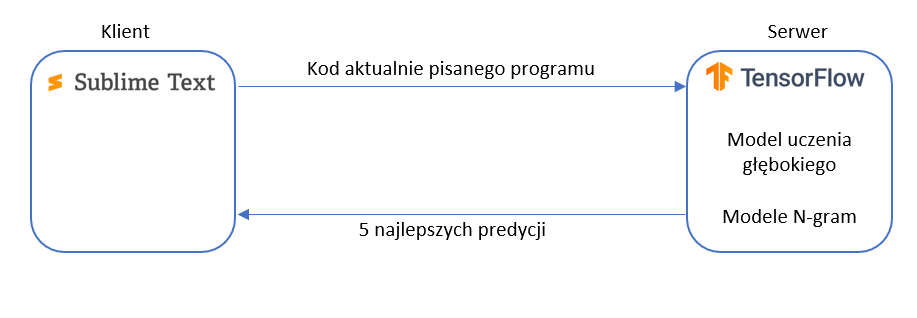
\includegraphics[width=450px, height=200px]{klient_serwer.png}
\end{figure}
\end{description}
\subsection{Obsługa}
Wtyczka po każdym naciśnięciu spacji, enter lub któregoś ze znaku specjalnego wysyła zapytanie do serwera składające sie z całego kodu aktualnie 
modyfikowanego programu, a w odpowiedzi uzyskuje wiadomość składającą sie z 5 najlepszych predykcji wykonanych przez model. Następnie użytkownik 
może wybrać którąś z sugestii poprzez naciśnięcie kombinacji klawiszy \begin{math}ctrl + i, i\in \{1,2,3,4,5\}\end{math}.
\begin{figure}[!h]
	% Znacznik \caption oprócz podpisu służy również do wygenerowania numeru obrazka;
	\caption{Działanie wtyczki}
	% dlatego zawsze pamiętaj używać najpierw \caption, a potem \label
    \label{fig:dzialanie_wtyczki}
    % Zamiast width można też użyć height, etc. 
    \centering 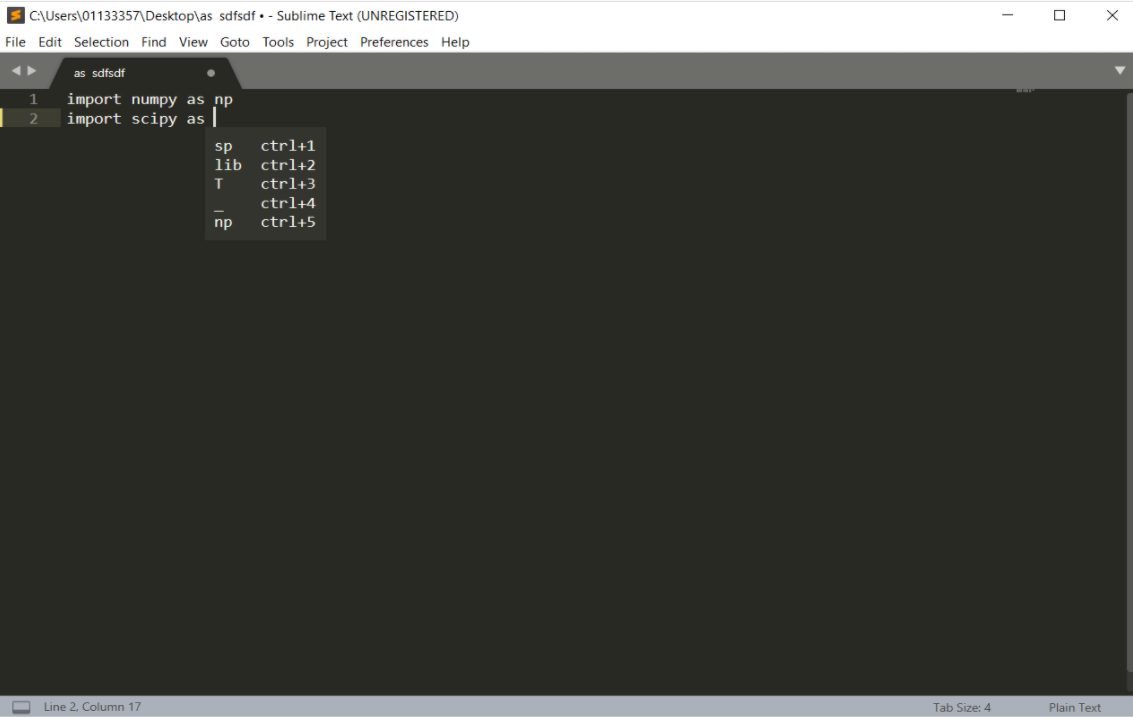
\includegraphics[width=450px, height=300px]{ss.png}
\end{figure}
\subsection{Czas odpowiedzi modelu}
Po wykonaniu 1000 zapytań do serwera odpowiedzialnego za wykonywanie predykcji, średni czas odpowiedzi wyniósł 18.8ms. W skład tej operacji 
wchodzi wysłanie zapytania do serwera lokalnego, tokenizacja danych, wykonanie predykcji oraz odesłanie odpowiedzi. Czas ten jest na tyle 
krótki, że nie ma żdanego wpływu na efektywność pisania kodu. 


